% \begin{figure}[t!]
%     \setlength{\belowcaptionskip}{-1em}
%     \centering
%     \subfloat[t][]{    
%     \resizebox{0.45\linewidth}{!}{\adjustbox{valign=b}{%
%     \begin{tabular}{lrrrr}
%         \hlineB{2}
%         Type& \rotatebox{90}{\txone~} & \rotatebox{90}{\txtwo} & \rotatebox{90}{\xavier~} & \rotatebox{90}{Total}\bigstrut\\\hlineB{2}
%         Latency & 6 & 9 & {5} & \cellcolor{gray05}20 \bigstrut[t]\\
%         Energy & 6 & 4 & {8} & \cellcolor{gray05}17 \\
%         Thermal & 5 & 2 & {2} & \cellcolor{gray05}9 \bigstrut[b]\\
%         \rowcolor{gray05} Total & 17 & 15 & 15 & \cellcolor{gray12} 47 \bigstrut\\ \hlineB{2}
%     \end{tabular}%
%     \label{tab:perf_faults_count}
%     }
%     }
%     }~
%     \subfloat[t][]{
%         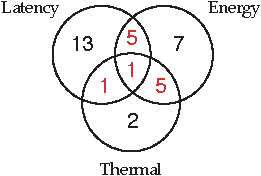
\includegraphics[width=0.45\linewidth, valign=b]{fig__venn.pdf}
%         \label{fig:perf_faults_venn}
%     }    
% \caption{\small non-functional faults in reported in NVIDIA Jetson\textsuperscript (gathered from NVIDIA developer forum). (a) Distribution across hardware, (b) Distribution across fault type ({\color[HTML]{CC3333} \bfseries red} indicate cases with multiple non-functional fault types).}
% \label{tab:perf_faults_summary}
% \end{figure}